% ---------------------------------------------------------------------
% EG author guidelines plus sample file for EG publication using LaTeX2e input
% D.Fellner, v1.17, Sep 23, 2010

\title[NetVis Network Traffic Visualization]
      {NetVis: a visualization tool enabling multiple perspectives of network traffic data}

% for anonymous conference submission please enter your SUBMISSION ID
% instead of the author's name (and leave the affiliation blank) !!
\author[Nicholls et al.]
       {J. Nicholls, D. Peters, A. Slawinski, T. Spoor, S. Vicol, J. Happa, M. Goldsmith and S. Creese
        \\
         Department of Computer Science, University of Oxford
       }

% ------------------------------------------------------------------------
% if the Editors-in-Chief have given you the data, you may uncomment
% the following five lines and insert it here
%
% \volume{27}   % the volume in which the issue will be published;
% \issue{1}     % the issue number of the publication
% \pStartPage{1}      % set starting page
%-------------------------------------------------------------------------
\begin{document}\addtolength{\parskip}{-0.25mm} %-0.25mm
\teaser{
\centering
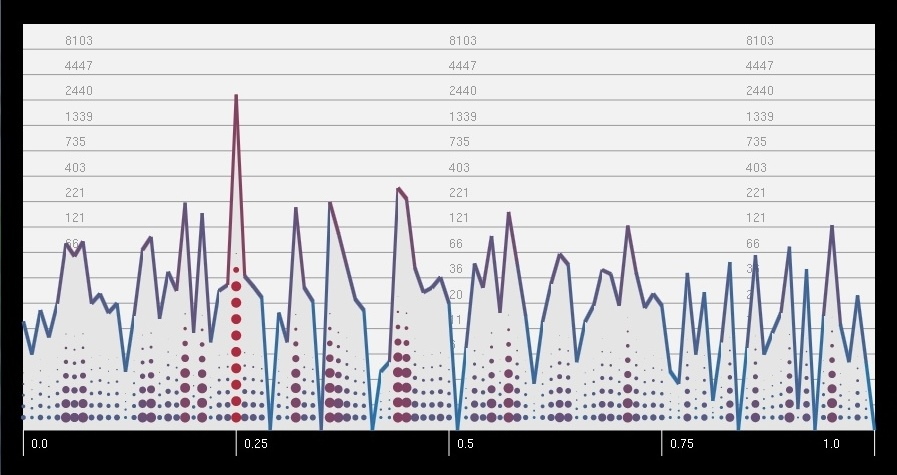
\includegraphics[width=0.251\linewidth]{materials/distribution-tease2}
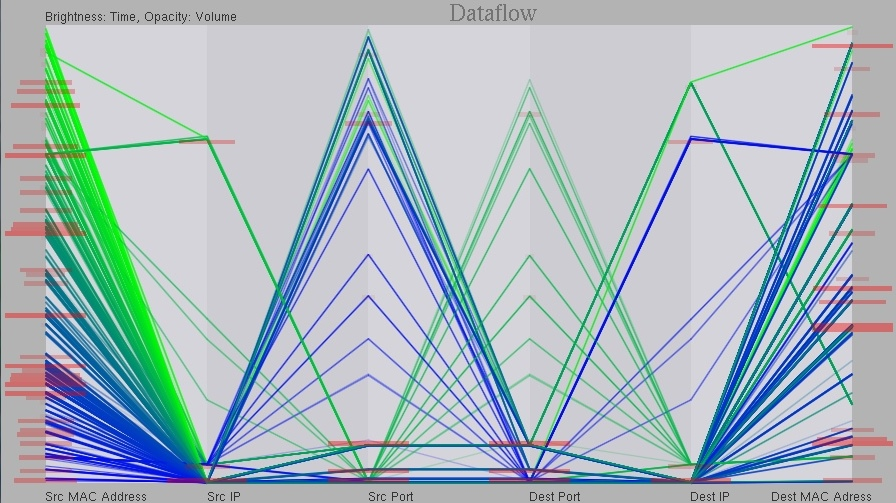
\includegraphics[width=0.25\linewidth]{materials/dataflow-tease2}
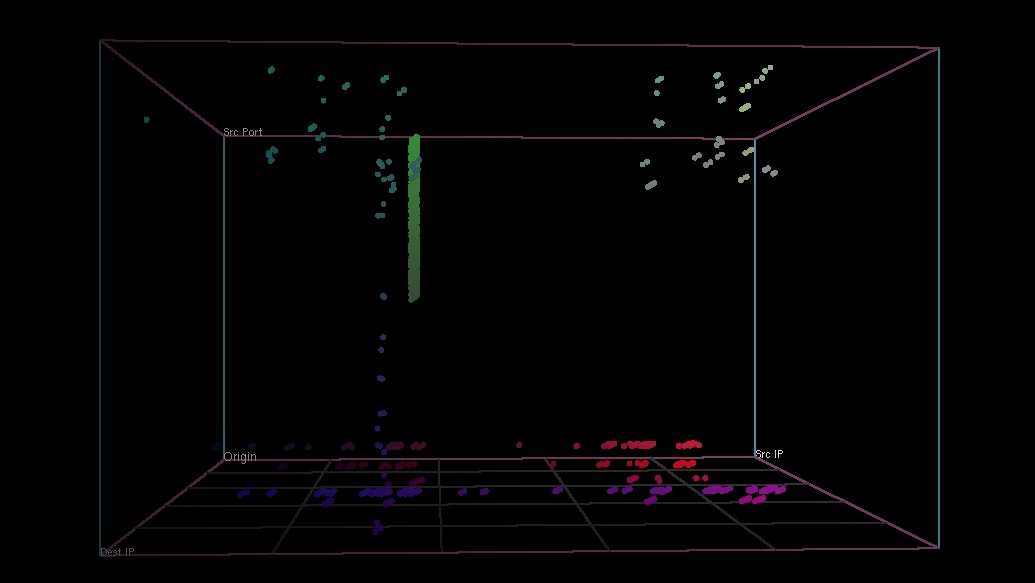
\includegraphics[width=0.25\linewidth]{materials/cube}

\centering
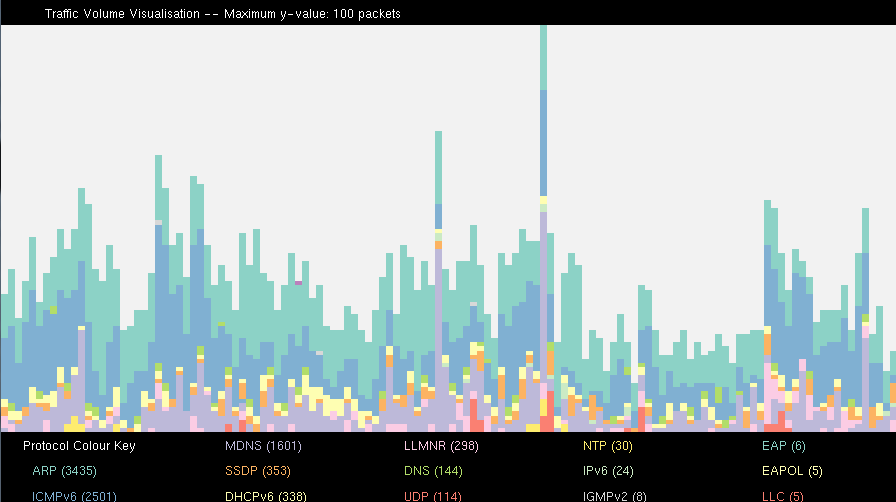
\includegraphics[width=0.25\linewidth]{materials/traffic-volume-tease2}
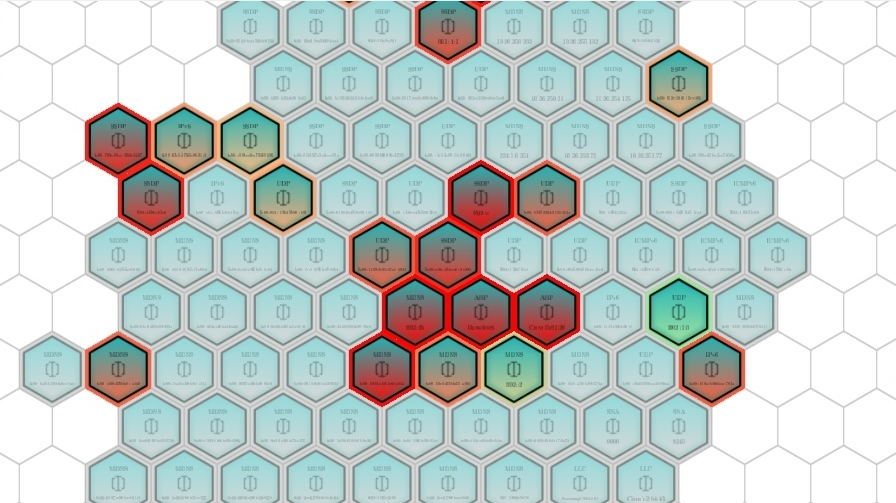
\includegraphics[width=0.25\linewidth]{materials/heat-map-tease2}
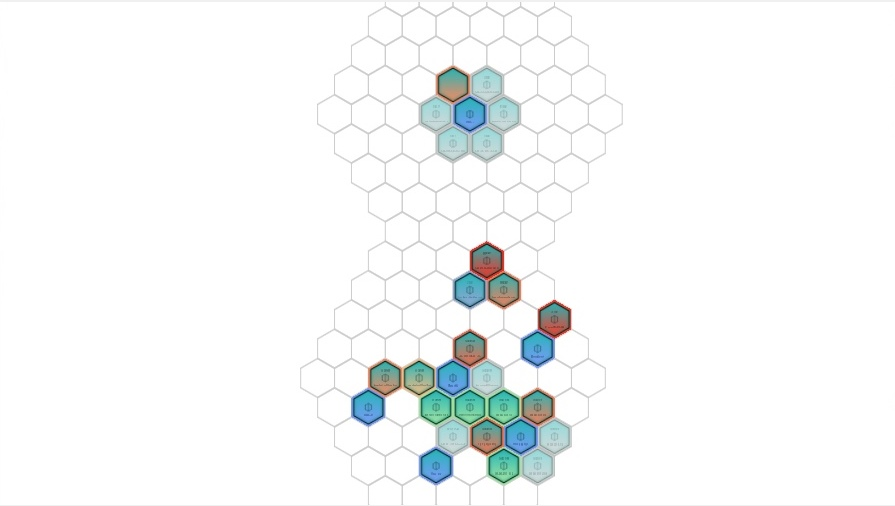
\includegraphics[width=0.25\linewidth]{materials/groups-tease2}

\centering
\caption{The suite of visualizations in NetVis. In order of appearance from top-left to
bottom-right: Attribute Distribution, Data Flow (Parallel Coordinate Plots), Spinning Cube of
Potential Doom, Traffic Volume, Heat Map and Activity Groups.}\label{fig:teaser} }

\maketitle

\begin{abstract}
Computer network traffic visualizations deliver improved understanding of pattern-of-life for
networks, and via such enhanced awareness can facilitate the detection of malicious traffic.
Existing tools often opt for graph or plot-based visualizations to detect patterns or outliers in
the data, but they still largely provide a segmented view of any data feed. In this paper we
present a novel framework designed to support multiple heterogeneous visualizations of network
traffic data. NetVis enables different visualizations that work in tandem to provide different
perspectives of the same data in real-time. As each visualization is modularly tied together it
enables a user to investigate on-going activity, or any subset of it, at their pace and based on
their priorities for further exploration. We currently support six visualizations, three are new and
three are based on existing literature (parallel coordinate plots, flowscan and spinning cube of
potential doom). Our results show that it is possible to use NetVis to detect unusual activity and
cyber attacks on a network. The framework is written to allow future visualizations to
be added straightforwardly.

\begin{classification} % according to http://www.acm.org/class/1998/
\CCScat{Computer Graphics}{I.3.8}{Applications}
\CCScat{Management of Computing and Information Systems}{K.6.5}{Security and Protection}
\end{classification}
% Keywords: Computer Security Visualization, Network Traffic, Scientific Visualization, Information
% Visualization
\end{abstract}

\section{Introduction} \label{sec:intro}
%Analysing and monitoring network traffic is an important part of network security. Since the amounts of data involved in this task are extraordinarily large, it can be hard to make effective use of them. Visualizations offer a solution: they give a compact representation of data to a human analyst who can use them to detect patterns in the network \cite{ware2012information}. An effective visualization of network traffic makes it easy to identify outliers while making clear the general patterns of network usage, and it will facilitate detection of intrusions and malicious activity.

In this paper, we present a set of visualization techniques that work in tandem to improve awareness of activities in ongoing network traffic passing through an analysts systems. They have been implemented in a robust application to provide an analysis framework for 
network activity in an interactive manner, enabling a deeper and more straightforward understanding of the data. Two of the visualizations are based on existing literature (parallel coordinate plots \cite{inselberg1985plane} and spinning cube of potential doom \cite{cube04}), whereas the four remaining visualizations are novel to this paper. These are referred to as: Attribute Distribution, Traffic Volume, Heat Map and Activity Groups.  

Time series data in the form of packet captures are processed in real-time and simultaneously rendered in multiple connected visualizations. The user can switch between the available representations of the data and change both the visualization's layout and the amount and type of the data displayed. The software is designed to make it easy to spot irregular activity and investigate it from multiple perspectives.

The framework aims to provide an environment in which situational awareness can more effectively be obtained. It is therefore flexible to the demands of the specific situation. New visualizations will in a natural way complement the existing ones: The underlying data processing engine provides a standard data basis which is shared by all displays.

The tools emphasize exceptions, show comparisons, and answer a wide variety of questions in a concise fashion. We want the user to generate good hypotheses in response to the visualized information. To achieve this, aids are given to the user to avoid cluttering displays with irrelevant data. In particular, we have implemented a filtering system which can be adjusted in response to changing situations.

Though the application's main purpose is to monitor current activity in the network, the same architecture can be used to forensically analyse recorded data. The system simulates the data records as if they represent a live network. This exploits the important dimension of time and makes it easier to understand recorded activity.

Monitoring and analysing network traffic is an important part of network security as it provides a
means to detect malicious activity on network systems. This is typically by detecting known attack
patterns or by seeking to understand normal pattern-of-life activity for the network and then
detecting deviations which might indicate presence of malicious events. As the amounts of data
to process increase substantially each year, it is becoming more and more difficult to make
effective analysis of on-going activity on a network. Visualizations offer a very useful solution:
they give a compact representation of data to a human analyst who can use them to detect patterns in
the network \cite{ware2012information}. Effective visualizations makes it easy to identify outliers
while making clear what general patterns are arising, facilitating detection of malicious activity.

In this paper, we present a framework implemented as a software application. Specifically, we are
interested in harnessing the ability of the human analyst to \textit{detect} unusual and possibly
malicious activity, and in supporting that analyst through the use of visualisations; in particular,
through the use of multiple visualisations from a single platform. We envisage an environment where
the analyst can easily switch between visualizations, exploring the dataset until a particular
visualisation resonates as \textit{showing} something of interest. Current approaches to supporting
analysts with visualizations are typically configured around proprietary Security Incident Event
Management (SIEM) environments, and so are by their nature limited in scope to a finite set of
visualizations. In contrast, our view is that the visualization should be working in tandem to
improve situational awareness and that we should not assume that there is any single optimal set of
visualizations which will work for all analysts in all operating conditions. For this reason we have
developed a framework which can easily support new visualizations as well as the tailoring of
existing ones.

We enable interactive analysis, we allow a deeper and more straightforward understanding of the data
by enabling an analyst to explore their raw datasets in a way that they deem appropriate given any
current situation. Time series data, in the form of packet captures, are processed in real-time and
simultaneously rendered in multiple connected visualizations. The user can switch between the
available representations and change both the visualization's layout and the amount and
type of the data displayed. The software is designed to make it easy to spot irregular
activity and investigate it using multiple perspectives. Three of the visualizations are based on
existing literature (\textit{Parallel Coordinate Plots} \cite{inselberg1985plane}, \textit{Flowscan}
\cite{plonka2000flowscan} and \textit{Spinning Cube of Potential Doom} \cite{lau2004spinning}). Some
of their limitations have been addressed in our implementations. The three remaining visualizations
are novel to this paper. These are referred to as: \textit{Attribute Distribution, Heat Map} and
\textit{Activity Groups}.

New visualizations can complement the existing ones: The underlying data processing engine provides a standard data basis which is shared by all displays. The tools emphasize exceptions, show comparisons, and answer a wide variety of questions in a concise fashion. We want the user to generate good hypotheses in response to the visualized information. To achieve this, we have implemented a filtering system which can be adjusted in response to changing situations. 

Though NetVis's main purpose is to monitor current activity in the network, the same
architecture could be used to forensically analyse recorded data. This allows us to exploit the
important dimension of time, making it easier to understand recorded activity in the context of a
digital investigation after the fact.

The remainder of the paper is divided into the following sections: Section \ref{sec:relatedwork}
summarises related work. Section \ref{sec:overview} provides an overview of NetVis's architecture
design. Section \ref{sec:visuals} describes each of the visualizations in detail, and Section
\ref{sec:workflow} describes our workflow paradigm with some example scenarios to demonstrate the
usefulness of our framework. A reflection on the utility of our methods and future work directions
can be found in Section \ref{sec:discussion} and the conclusion is presented in Section \ref{sec:conc}.

\section{Related Work} \label{sec:relatedwork}
Visualization approaches provide different perspectives view of a dataset based on criterias of interest. Some of the techniques favour graph-based representations, port-scanning activity characteristics, network traffic patterns, payload characteristics or event-log forensics. More specifically, these could include use of parallel coordinate plots \cite{picviz}, treemaps \cite{johnson1991tree}, geolocation \cite{prole2008wireless} and visual firewall \cite{lee2005visual}. 

Rumint \cite{rumint} and Wireshark \cite{wireshark} are examples that can be used for traffic forensics. For analysing network traffic patterns a variety of strategies have been proposed including traffic volume \cite{plonka2000flowscan} and raw data relationships \cite{lau2004spinning}. Best et al. \cite{best2010} also demonstrated the usefulness of tools such as Traffic Circle, CLIQUE and MeDiCi to improve situational awareness by exploring raw dataset through visualization.

Conti \cite{Conti} and Marty \cite{marty2009applied} provide a detailed discussion on this topic, while Zhang et al. \cite{zhang2012survey} presented a survey overviewing the techniques. Other tools and visualization techniques can be found in the SecViz.org \cite{SECVIZ} gallery. 

\subsection{Motivation}
While many tools exist to improve aspects of network traffic data understanding, few works have discussed how multiple visualization techniques can work together to deliver an improved understanding of network activities. NetVis addresses this problem by showing how multiple heterogeneous of visualizations approaches can work together. Three are improvements on known visualization techniques (Parallell Coordinate Plots, FlowScan and Spinning Cube), while the latter three are new visualizations for network traffic.

\section{NetVis Architecture}\label{sec:overview}
NetVis is a Java application which uses OpenGL (JOGL) to draw visualizations and Swing to provide a
Graphical User Interface (GUI). In designing the application, maintaining extensibility and keeping
a modular programming style was a large focus. It is now straightforward to add support for
additional input data formats, or to develop a new visualization that utilises the same data
processing engine.

Packet data is transferred to the application as a CSV packet capture file. NetVis uses a file
format that can be directly obtained from the packet analyser Wireshark \cite{wireshark}. NetVis
will process each packet and analyse its fields which includes: \textit{timestamp, information about the packet's source (IP, hardware (MAC) address, port), information about the packet's destination,
communication protocol, and the packet length in bytes}. The current version of NetVis does not
process the content of packets. 

% All capture files are provided to the application as CSV files with the following headers;
% - No. Packet number
% - Time Time elapsed since first packet (seconds)
% - Source IP Source IPv4/6 address
% - Source HW Source hardware (MAC) address
% - Source Port Source port
% - Dest IP Destination IPv4/6 address
% - Dest HW Destination hardware (MAC) address
% - Dest Port Destination port
% - Protocol Communication protocol
% - Length Packet length (bytes)
% - Info Detected description of packet purpose

A convenient feature of the data input system is a time control system. The CSV file is processed as
if its packets would arise in a live network. The user can choose to speed up or slow down the
speed with which packets are fed into the application, can pause processing, or skip towards the end
of the data record. This is helpful in analysing the data since critical time intervals can be
analysed in more detail. The application is set up in such a way that it is also easy to use the
activity of a live network as its input source. 

The input data is processed in a data controller that supplies visualizations and the user
interface with packet data. If the user has chosen to apply filters to the data, the data controller
only directs the filtered data stream to the rest of the application, so that all parts share a
common data source.

NetVis includes a data filtering system that allows users to select a subset of processed packets
which exhibit features which the user specified to be of interest. The application supports two
types of filters: filters that the user explicitly defines, and filters applied on-the-fly from
within the visualizations. Both types are applied to all visualizations and information displayed,
and they can be adjusted at any time without losing prior data.

There are a variety of filter controls. First, there is a menu for filtering by transit protocol.
By default, all protocols are selected and therefore included. Protocols are sorted into menus by
protocol family, appearing in multiple places where appropriate. Second, there is a control to
select the range of ports the application uses, which defaults to the maximum port range.  The
source and destination ports can be set separately, enabling a user to view all data
entering/exiting a port as desired.  Third, there are IP and MAC address filters.  These work on a
blacklist/whitelist system, allowing a user to only view packets to or from a particular set of
addresses, or to ignore packets going to or from a different set.  This enables a user to, for
instance, ignore traffic from sources they know are irrelevant or focus only on an address that is
causing concern.

The packet attributes that are processed by NetVis do not share a common scale, nor are they
necessarily orderable. It is, however, desirable to map some of these properties into a shared
representation which allows a more intuitive grasp of the distribution of attributes. We achieve
this by processing the packets in a `normalising' system. This system keeps track of the used values
and maps them into the interval $[0,1]$. In this way all normalised packets can be displayed in
relation to a number axis. This representation is used in three different visualizations. Each
normaliser is able to create a temporary filter in the application that will filter its
corresponding attribute on a certain range. Since the normalising class is in control of its filter
this creates a zooming effect based on the range of the filter: the lower bound is normalised to 0,
the upper bound to 1.

%Modularity: \textbf{[Make this better.]}
\begin{figure}[htb]
   \centering
   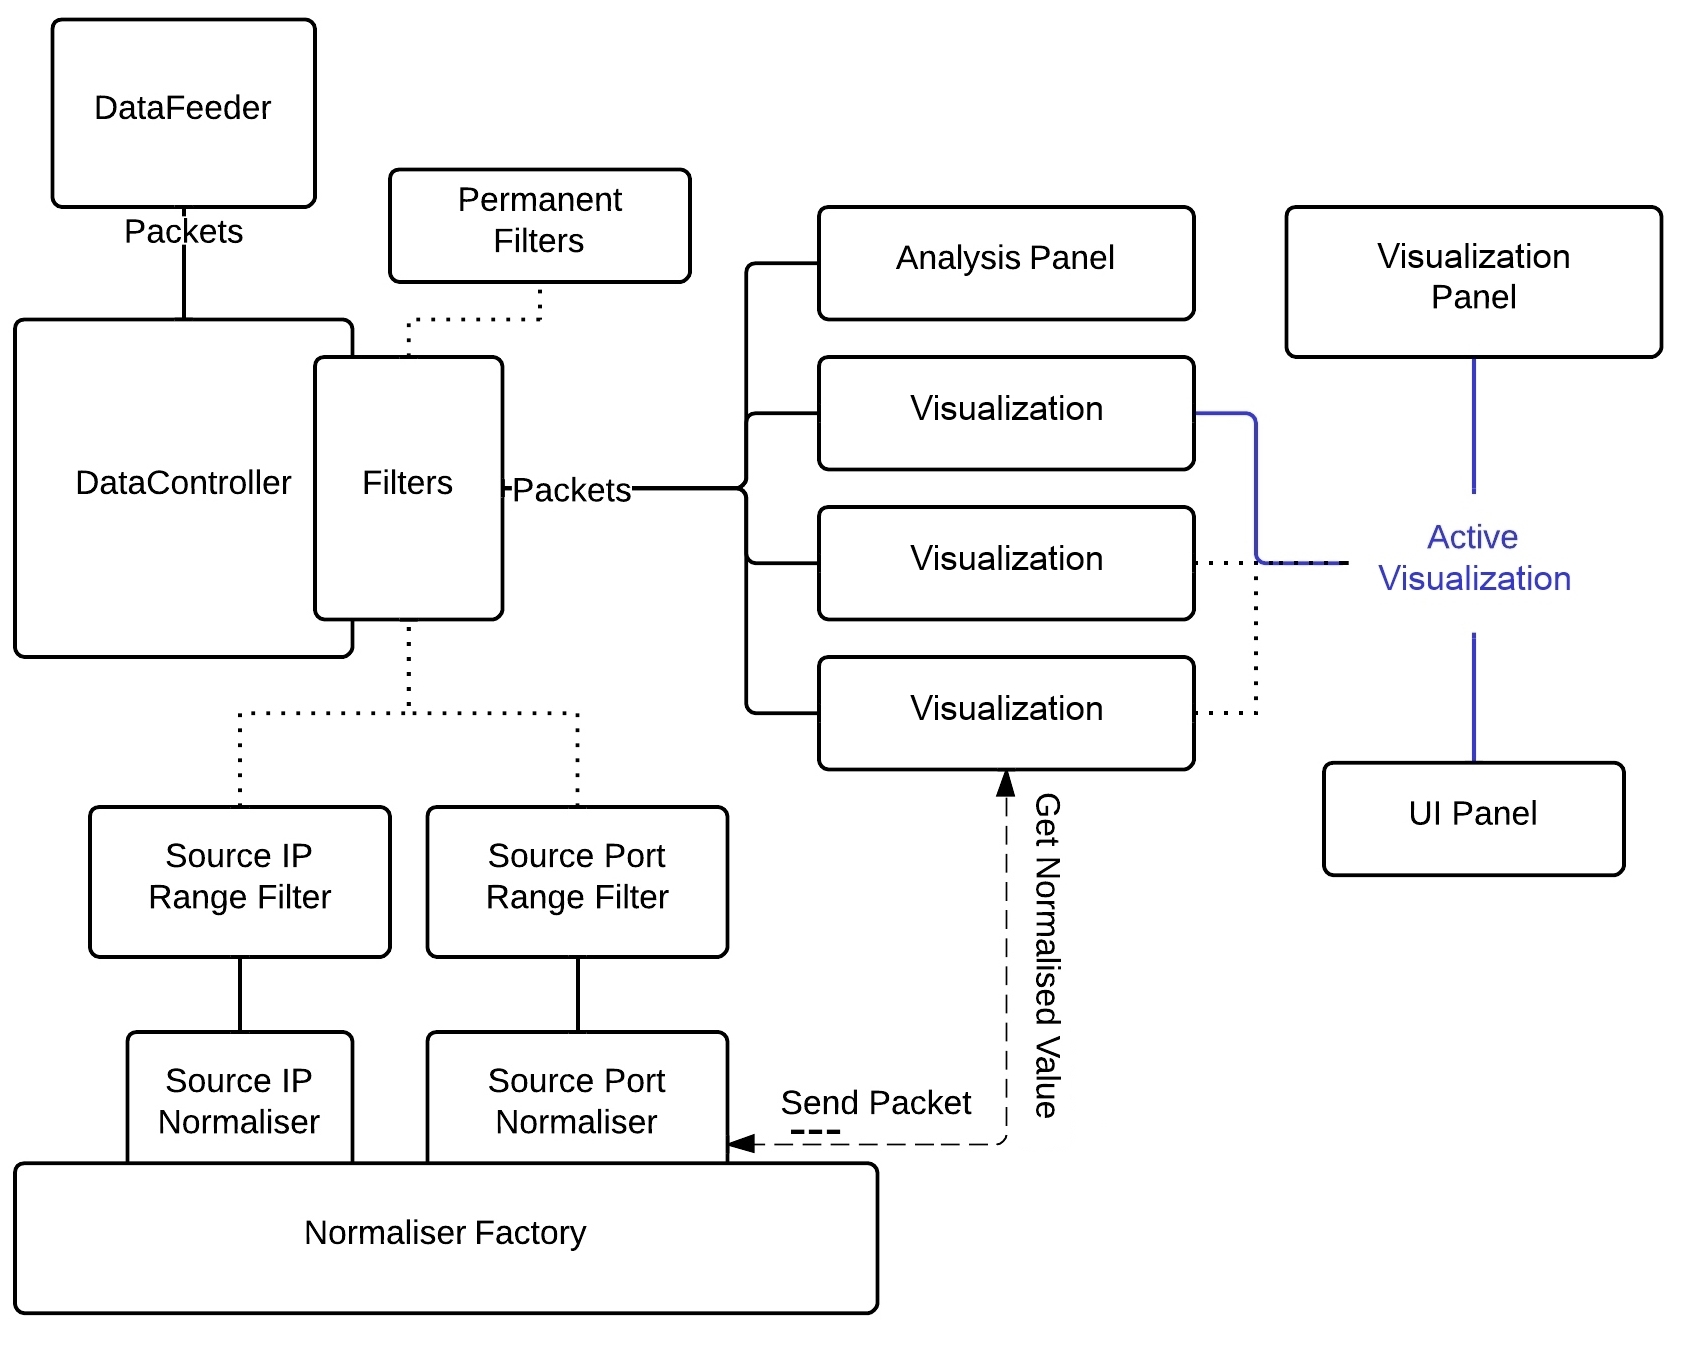
\includegraphics[width=\linewidth]{materials/architecture.jpg}
   \caption[Architecture]{\label{fig:architecture}
         Diagram overviewing the architecture of NetVis.}
\end{figure}

The application is designed to be extensible. Adding a new visualization is a matter
of adding it to the application's list of those available, which will keep it up-to-date
as packets come in and are filtered. The same is true for filters and normalisers. A diagram
overview of the system's architecture can be found in Figure \ref{fig:architecture}.

% Adding a filter would result in its controls automatically
% being included in the right panel and all packets would then be filtered according to the criteria
% it specifies.  Adding a normaliser would cause it to be integrated with the Spinning Cube,
% Dataflow and Attribute Distribution visualizations.  This modularity extends even so far as data
% input.  If a class were written to accept packets from a different source, it would be trivial to
% switch the application to use this class.

\section{NetVis Visualizations} \label{sec:visuals}
\subsection{Graphical User Interface}
The displayed (current) visualization occupies most of the user interface and can be maximised to
fill all screen space. A displayed visualization may use both multi-dimensional systems (such as
parallel coordinates) to give an overview and lower-dimensional visualizations to provide more
detail. This encourages an understanding of network activity that is both broad and detailed. Other
panels of the GUI occupy the right and bottom sections of the window to allow user input and
detailed information to be viewed, see Figure \ref{fig:layout}. {\textbf{Key}}: 1) Visualization, 2)
Analysis Panel, 3) Context Panel, 4) Visualization-specific options, 5) General data filters and 6)
Data source identifier.

\begin{figure}[htb]
   \centering
   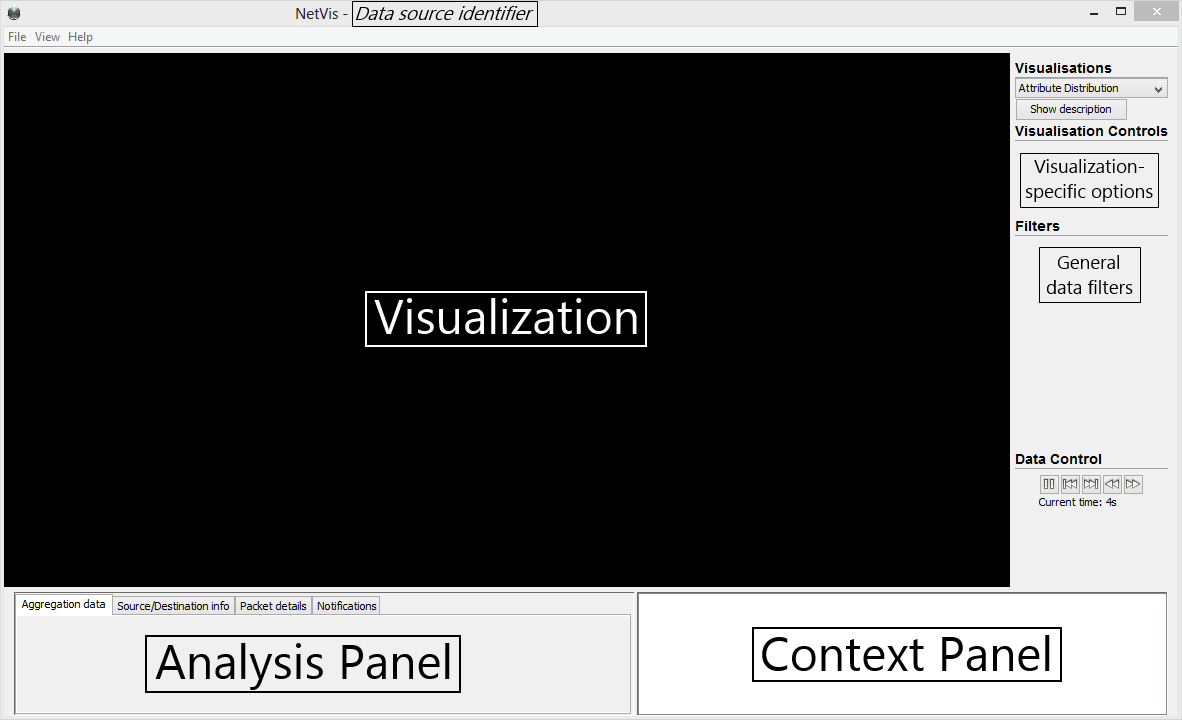
\includegraphics[width=\linewidth]{materials/layout-diagram.png}
   \caption[GUI]{\label{fig:layout}
         An overview of the GUI layout of NetVis.}
\end{figure}

\subsubsection{GUI: Right Panel}
The right panel is aimed at providing the user with options to adapt the shown data. Choice of
visualization is presented to the user by a list in the top of the right panel, followed underneath
by options specific to that visualization, and then by general filters to refine the processed data.
If a recorded data source is active, time controls are displayed on the right panel to allow the
user to adjust the speed at which data is processed and visualised by pausing, doubling or halving
the current data rate.

\subsubsection{GUI: Bottom Panel}
The bottom panel shows fine and aggregate details of the processed data. To fit the large amount of
data available into such a limited space, a tabbed pane is used on the left to categorise distinct
types of data. The right section of this panel contains a `Context Pane', which shows further detail
of selected data on demand. The left `Analysis' panel and the right `Context' panel are split in two
by a split pane, so the user can modify the proportion of each they wish to see.

% Compressed and merged the below paragraphs, I think it's important to explain
% about user messages, it's an important part of the interface.

Window tools, an exclusive-mode full screen option and the facility to select a new data source are
all accessed by the main menu bar. Messages to the user come in the form of warning dialogues for
user or program errors, notifications in the bottom `Analysis' panel for program notifications, and
text messages in the bottom `Context' panel for help messages and suggestions.

\subsection{Visualization: Attribute Distribution}
%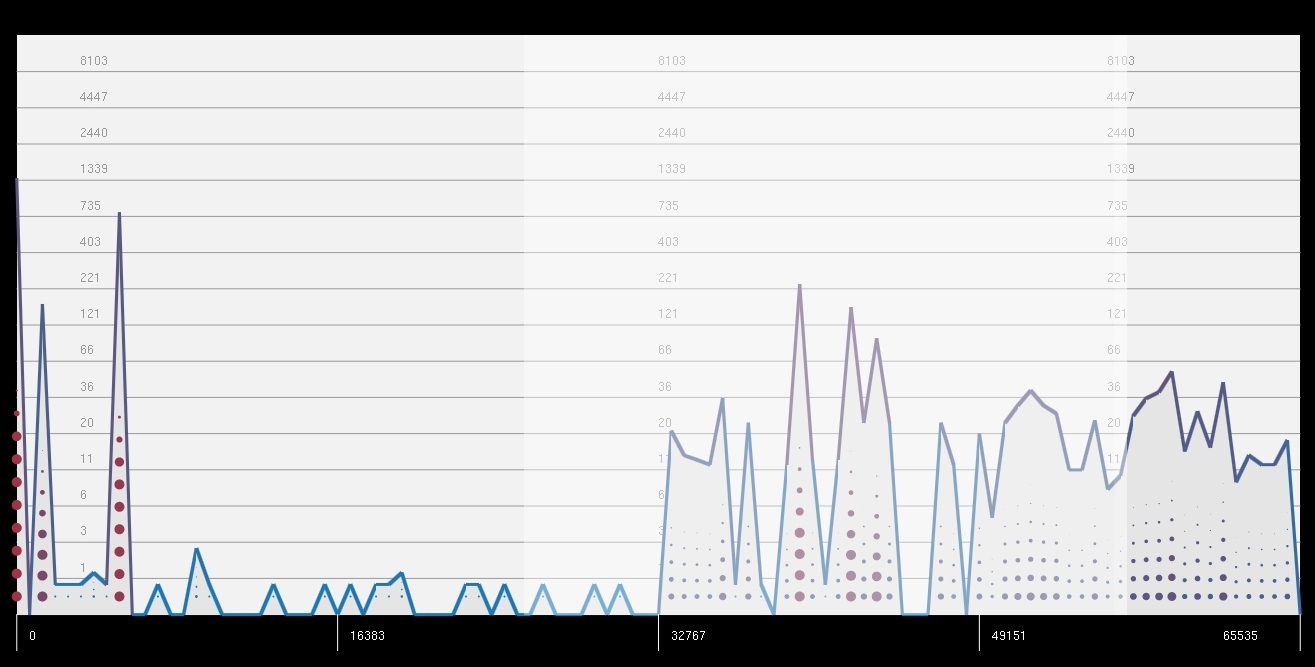
\includegraphics[width=\linewidth]{materials/distribution.jpg}

The most common need in the analysis of network traffic is to get information on the distribution of certain features of the packets. For the graph constructed here, the user selects such a feature (e.g., ports or destination IPs). A logarithmic line graph is then drawn, and (as with all visualizations in the application) updated in real time. A logarithm is applied to assist in detecting spikes.

A second layer of the visualization is presented to the user simultaneously: Circles under the line graph indicate the actual distribution (without a logarithm applied) through their area. Furthermore, all lines and circles are colour-coded to give extra signals of the volume of traffic. Red elements are under heavier load.

All these features have a single purpose: make the analyst understand what is going on, and to make obvious any anomalies.

This visualisation makes active use of the normalisers described above. It also allows the user to click-and-drag along interesting data which then automatically applies a filter to the data so that all visualizations focus on this user-selected area of interest.

The most common need in the analysis of network traffic is information on the distribution of
certain features of the packets. For the graph constructed here, the user selects such a feature
(e.g., ports or destination IPs). A logarithmic line graph is drawn and (as with all visualizations
in the application) updated in real time. A logarithm is applied to assist in detecting spikes. A
screenshot of the Attribute Distribution visualization can be seen in Figure \ref{fig:distribution}.

\begin{figure}[htb]
   \centering
   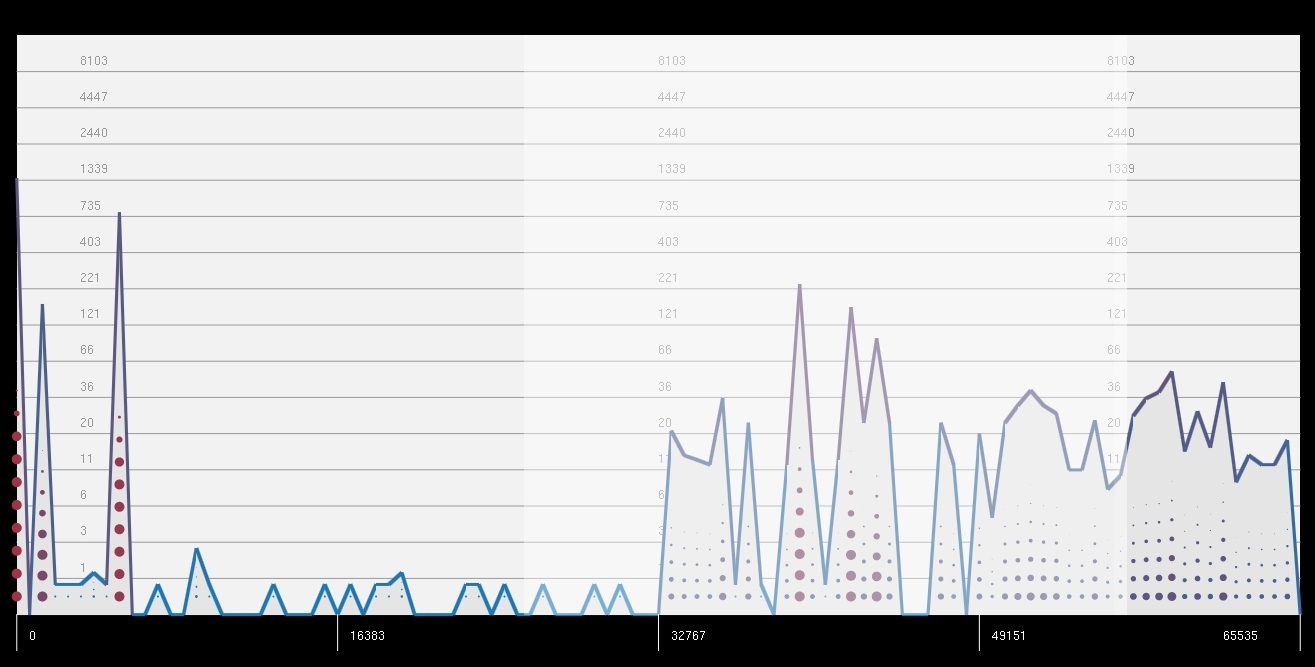
\includegraphics[width=\linewidth]{materials/distribution.jpg}
   \caption[Dataflow]{\label{fig:distribution}
         Attribute Distribution visualization.}
\end{figure}

A second layer of the visualization is presented simultaneously: circles under the line graph
indicate the actual distribution (without a logarithm applied) through their area. Furthermore, all
lines and circles are colour-coded to give extra signals of the volume of traffic. Red elements are
under heavier load. The visualization makes active use of the aforementioned normalisers. It also allows users to click-and-drag along interesting data to zoom into. Internally this means that a filter is applied and all visualizations show only the selected packets for closer examination.

\subsection{Visualization: Data Flow}
%The Data Flow visualization applies the idea of parallel coordinates proposed by \cite{inselberg1985plane} to network traffic. Following the principles layed out in \cite{fliggnetwork} the visualization shows the `flow' of each packet, representing each as a line through the parallel coordinates. This provides an informative view of the whole traffic in the network. It visualises the distribution of various packet attributes while also giving an intuitive insight into relationships and correlations between distinct aspects of the packets.

Lines representing packets are coloured based on their value in some coordinate. They fade out based on how old the packet is, thereby placing focus on newer developments in the network. 

A common criticism of parallel coordinate plots is that they make it hard to interpret data that is uniformly distributed between coordinates or that is very concentrated around few values \cite{marty2009applied}. Our implementation addresses these concerns using animation. Lines representing new packets are randomly pertubed and move subtely. This makes it easier to spot whether a colourful line represents one or more packets. The animation allows the user to distinguish between single packets and concentrated groups of packets with the same characteristics.

For example, if multiple requests to a server came from a single MAC address through the same ports and using the same protocol, in a non-animated visualization they would all be represented by the same line. A user would erroneuosly interpret this as a single request. Adding randomness makes the pack of requests more visible without significantly impacting the accuracy of the data representation.

Hovering over one coordinate displays a scale for the attribute it represents. Clicking transfers you to the distribution visualisation showing the distribution of that particular attribute.

The Data Flow visualization applies the idea of parallel coordinates proposed by
\cite{inselberg1985plane} to network traffic, see Figure \ref{fig:dataflow}. Following the
principles in \cite{fliggnetwork} the visualization shows the `flow' of each packet, representing
each as a line through the parallel coordinates. This provides an informative view of the whole
traffic in the network. It visualises the distribution of various packet attributes while also
giving an intuitive insight into relationships and correlations between distinct aspects of the
packets. 

\begin{figure}[htb]
   \centering
   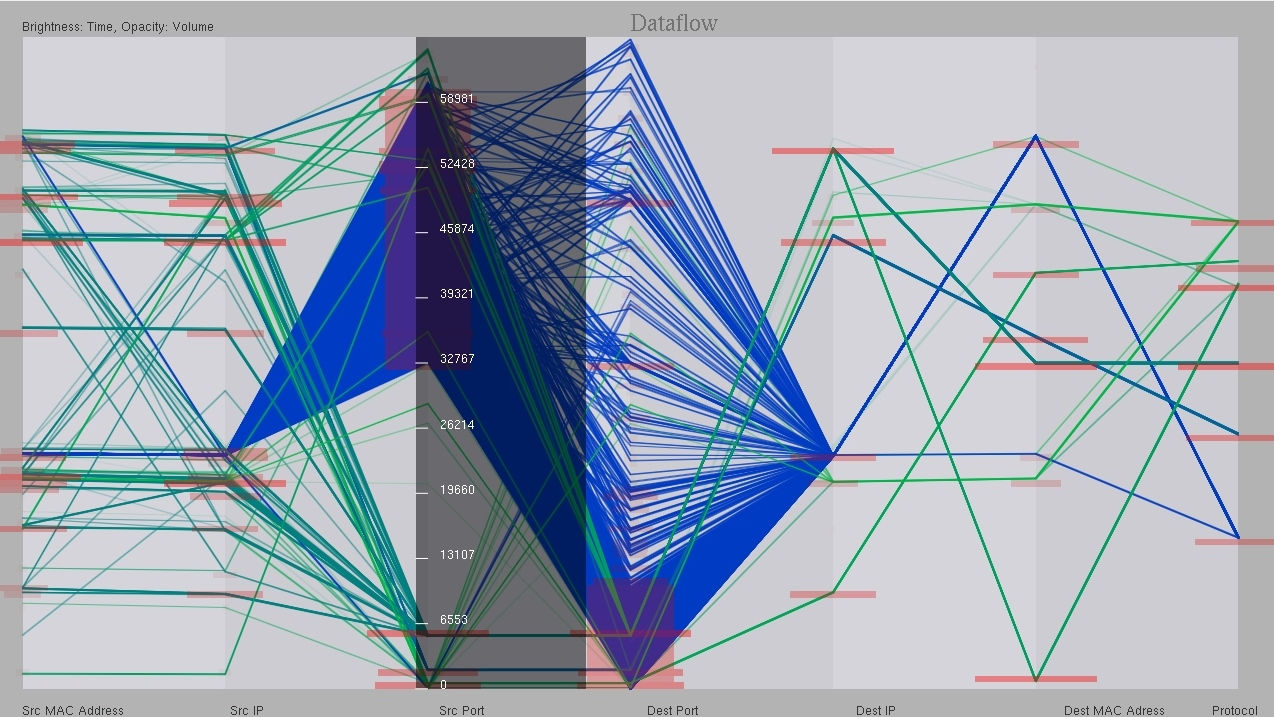
\includegraphics[width=\linewidth]{materials/dataflow.jpg}
   \caption[Data Flow]{\label{fig:dataflow}
         Data Flow visualization inspired by parallel coordinate plots \cite{inselberg1985plane}.}
\end{figure}

Lines representing packets are coloured based on their value in some coordinate. They fade out based
on how old the packet is, thereby placing focus on newer developments in the network.

A common criticism of parallel coordinate plots is that they make it hard to interpret data that is
uniformly distributed between coordinates or that is very concentrated around few values
\cite{marty2009applied}. Our implementation addresses these concerns using animation. Lines
representing new packets are randomly perturbed and move slightly. This makes it easier to spot
whether a line represents one or more packets. The animation allows the user to distinguish between
single packets and concentrated groups of packets with the same characteristics.

Suppose that multiple requests to a server come from a single MAC address through the same ports and
using the same protocol. A non-animated visualization would represent all these requests as a single
line. A user would erroneously interpret this as a single request. Adding randomness makes the pack
of requests more visible without significantly impacting the accuracy of the data representation.

The Data Flow visualization is closely tied to the previously described Attribute Distribution
visualization. If a coordinate shows an unusual distribution (say a uniform use of ports in a
certain range), then a single click on the packets in this coordinate will show the Attribute
Distribution log plot which allows direct access to filtering option. Hovering over packets also
displays further contextual information.

\subsection{Visualization: Spinning Cube}
%The Spinning Cube is an implementation of an existing visualization tool known as the spinning cube of potential doom\footnote{See \url{www.kismetwireless.net/doomcube/}}.
It�s displays packets as dots inside a spinning cube. Their 3D position is based on 3 packet attributes. (eg. x-axis $\Rightarrow$ Source Port / y-axis $\Rightarrow$ Destination Port / z-axis $\Rightarrow$ Source IP). The 3 coordinates are customisable.

\textbf{[make nicer]}

The Spinning Cube is a three-dimensional scatter plot that displays packets as dots inside a
rotating cube. The position of the dot is determined by its packet's attributes. This could be the
combination of source port, destination port, and source IP but also any other choice of packet
attribute, see Figure \ref{fig:cube} for a screenshot.

\begin{figure}[htb]
   \centering
   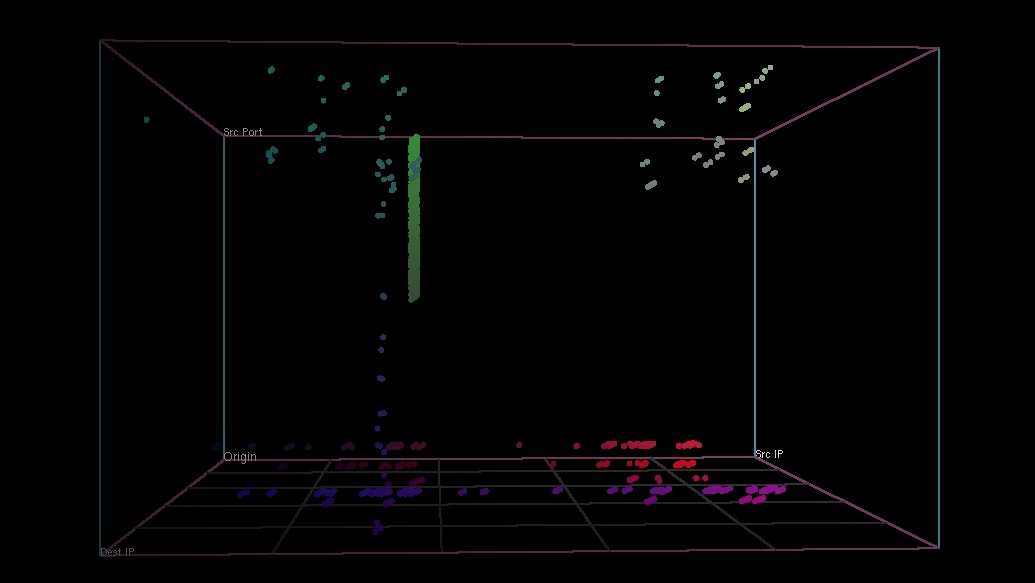
\includegraphics[width=\linewidth]{materials/cube.jpg}
   \caption[Spinning Cube]{\label{fig:cube}
         Spinning Cube of Potential Doom \cite{lau2004spinning}.}
\end{figure}

The visualization is an implementation of an existing visualization tool known as the Spinning Cube
of Potential Doom \cite{lau2004spinning}, but it offers additional controls for the user. In
particular, the axes can be chosen to represent arbitrary packet attributes that the user specifies.

To ensure good distinguishability of individual packets, we use the same principle of randomness as
in the Data Flow visualization. Every point is animated and perturbed. In this way, multiple packets
with the same attributes do not occupy the same pixel in the cube. It is thus easier to spot the
packet density of an area in the cube.

\subsection{Visualization: Traffic Volume}
%The Traffic Volume visualization is inspired by the `FlowScan' graph
(\url{www.caida.org/tools/utilities/flowscan/}). It is realised as a stacked
bar chart which displays the volume of data arriving in each time interval.
Each column is segmented into segments with heights proportional to the total
number of packets transmitted for each protocol.
In addition, the column segments are colour-coded and can be cross-referenced
with a protocol key underneath the visualization itself.

To help distinguish between different protocols, colours are selected from a
colour palette which provides colours from a qualitative colour scheme.
The objective of this visualisation is to allow users to see at a glance if a
particular protocol is being exploited in the network. The increase in both
column height and colour proportion should draw attention to any protocol which
becomes overburdened.

A control panel is provided in the right panel for the purpose of adjusting the
number of time intervals displayed at once on the x-axis. The y-axis scales
automatically to fit the relevant data.

The Traffic Volume visualization is inspired by the `FlowScan' graph \cite{plonka2000flowscan}. The
objective is to allow users to see at a glance if a particular protocol is being exploited in the
network. It is realised as a stacked bar chart which displays the volume of data arriving in each
time interval. Each column is segmented into sections with heights proportional to the total number
of packets transmitted for each protocol. In addition, the column segments are colour-coded and can
be cross-referenced with a protocol key underneath the visualization, see Figure
\ref{fig:traffic-volume} for a screenshot.

\begin{figure}[htb]
   \centering
   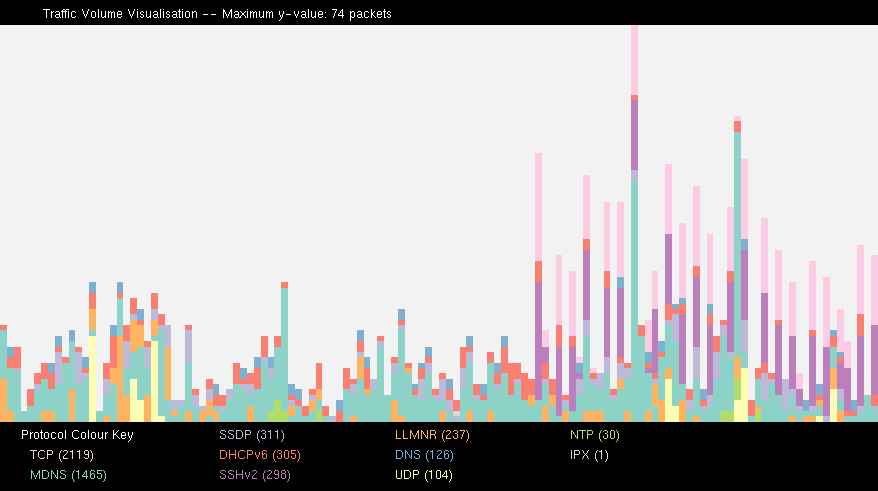
\includegraphics[width=\linewidth]{materials/traffic-volume.png}
   \caption[Traffic Volume]{\label{fig:traffic-volume}
        Traffic Volume visualization, inspired by FlowScan \cite{plonka2000flowscan}.}
\end{figure}

To help distinguish between different protocols, colours are selected from a palette which provides
colours from a qualitative colour scheme. The increase in both column height and colour proportion
should draw attention to any protocol which becomes overburdened. For instance, if a network
saturated with TCP traffic suddenly becomes flooded with DNS requests, the drastic change in colour
will alert the user to the change in circumstances. 

A control panel is provided in the right panel for adjusting the number of time intervals displayed
at once on the x-axis. The y-axis scales automatically to fit the current data.

\subsection{Visualization: Heat Map}
%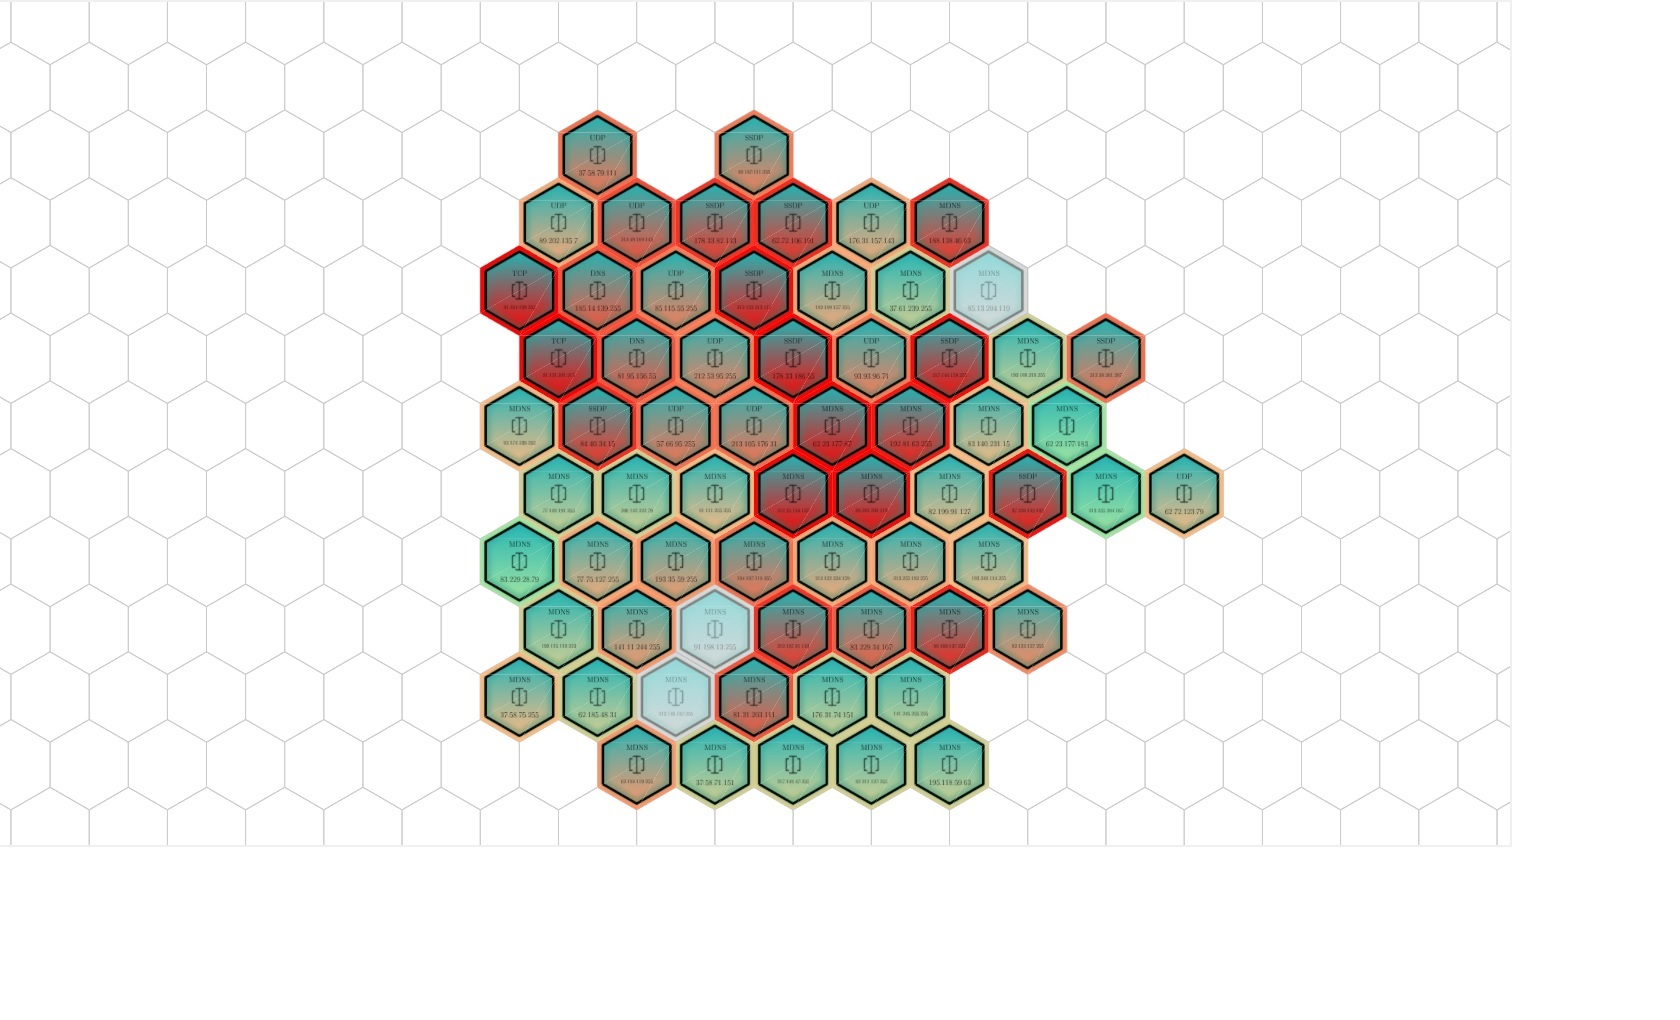
\includegraphics[width=\linewidth]{materials/heat-map.jpg}
The Heat Map visualization uses a hexagonal map to display a compacty cluster of nodes.
Each machine found to be communicating in the analysed network will be represented as a node.
The activity of a specific machine in the network is represented by the colour of the 
corresponding hexagon. As more and more traffic arises, nodes representing the machines that
send and reveive data ``heat up'' and, as the time passes, ``cool down''.
The hexagonal grid is being filled in a compact manner - new nodes are place outside of 
the already displayed nodes. The relative position of the map elements in this visualization
does not play a role on default. There is a way to sort the nodes so that they form a radial 
gradient - the more ``heated up'' will be sorted to the middle.

This visualization helps a user find machines that are most active in the network.
It gives a quick overview of the number of the clients and how many of them are currently active.
Additionaly every node presents some information, such as the machine's most commonly used protocol.
This lets users do some basic data selection choices easily. For example: if some other visualization
is being obscured by too much data from one specific machine, or too much data of some protocol,
the user can look at the heatmap and find out what filters to apply to make the overview of the situation
more clear.

The Heat Map visualization uses a hexagonal map to display a compact cluster of nodes.
Each machine found to be communicating in the analysed network will be represented as a node.
The activity of a specific machine in the network is represented by the colour of the 
corresponding hexagon. As more and more traffic arises, nodes representing the machines that
send and receive data ``heat up'' and, as the time passes, ``cool down''.
The hexagonal grid is filled in a compact manner - new nodes are place outside of 
the already displayed nodes. The relative position of the map elements in this visualization
does not play a role on default. There is a way to sort the nodes so that they form a radial 
gradient - the more ``heated'' will be sorted to the middle. See Figure \ref{fig:heatmap}
for a screenshot.

\begin{figure}[htb]
   \centering
   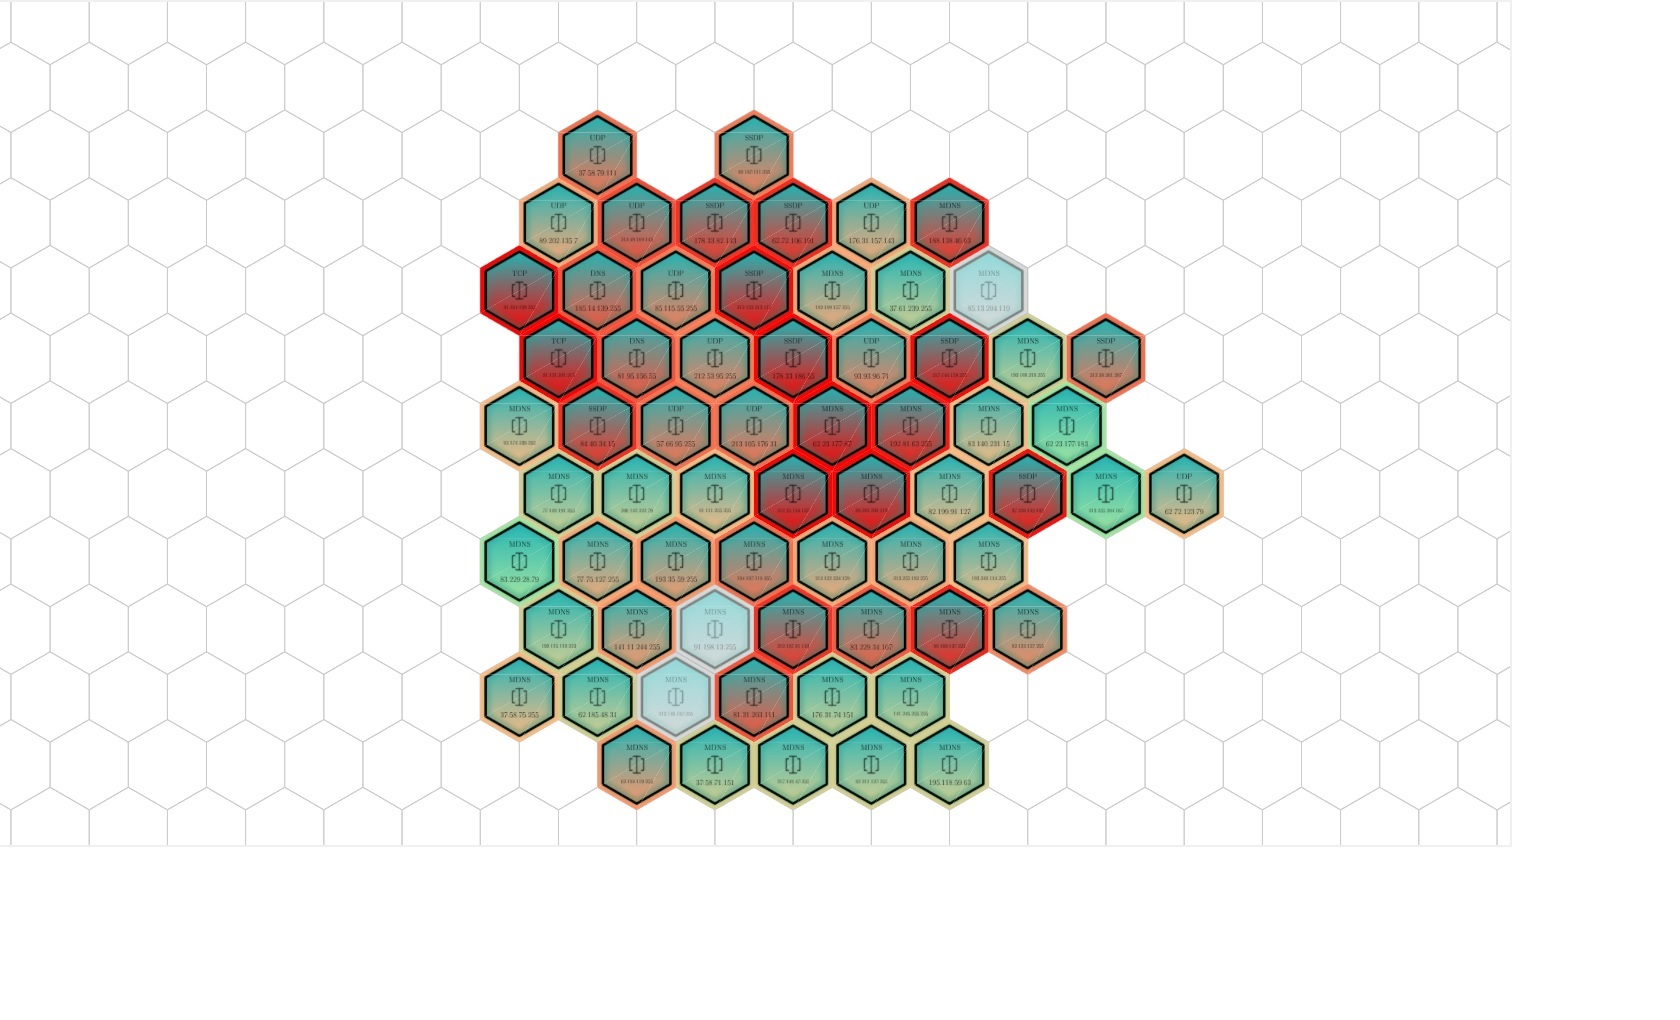
\includegraphics[width=\linewidth]{materials/heat-map.jpg}
   \caption[Heat Map]{\label{fig:heatmap}
         Heat Map visualization.}
\end{figure}

This visualization helps a user find machines that are most active in the network.
It gives a quick overview of the number of the clients and how many of them are currently active.
Additionally every node presents some information, such as the machine's most commonly used protocol. This lets users do some basic data selection choices easily. For example: if some other visualization is being obscured by too much data from one specific machine, or too much data of some protocol, the user can look at the heatmap and find out what filters to apply to make the overview of the situation more clear.

\subsection{Visualization: Activity Groups}
%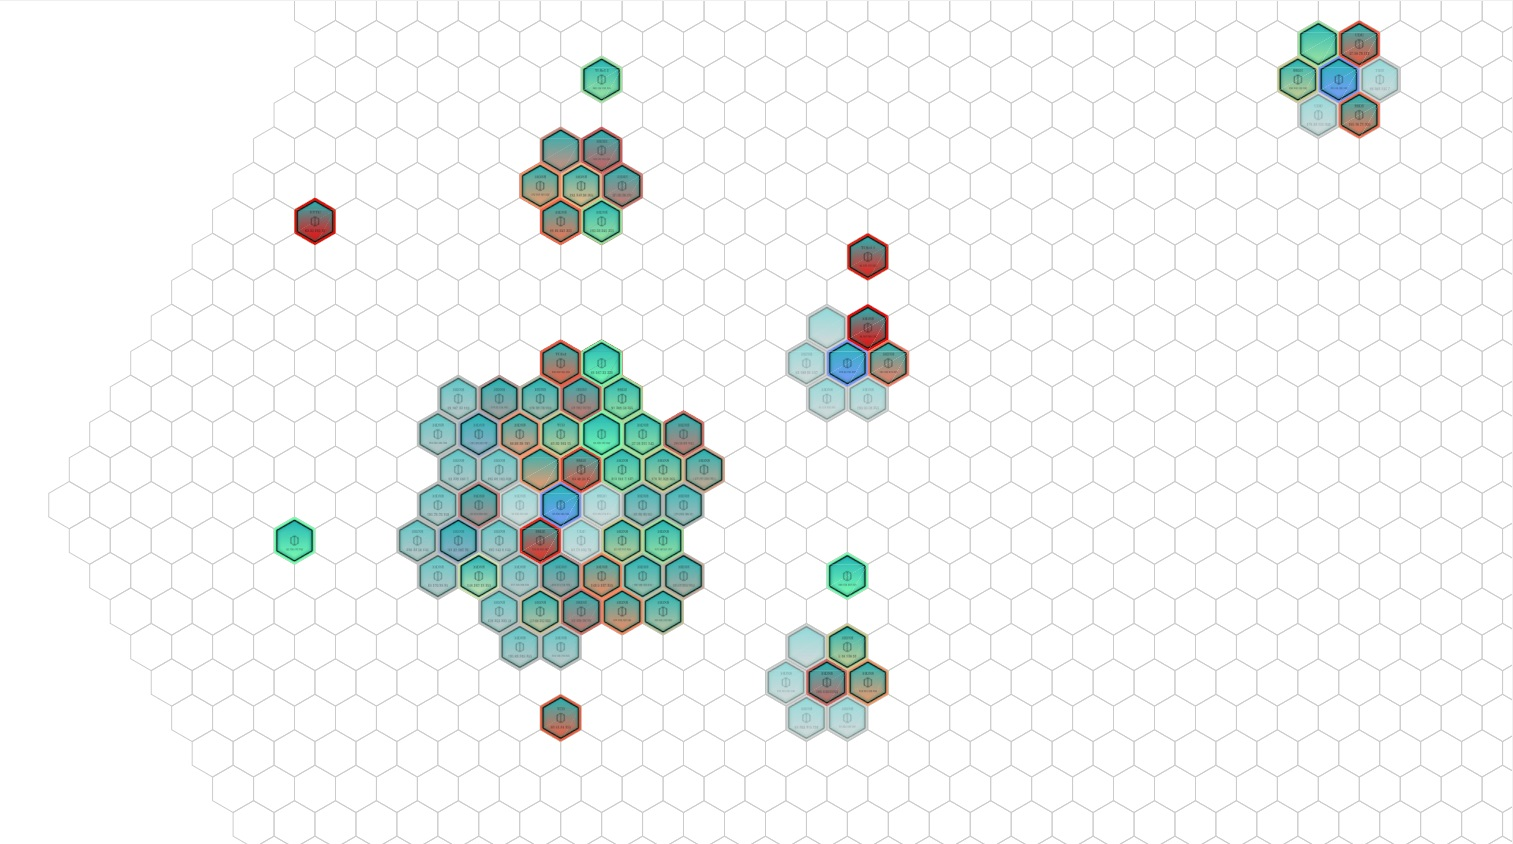
\includegraphics[width=\linewidth]{materials/groups.jpg}
Expanding on the hexagonal grid, this visualization employs two important visual factors:
size and proximity.

As the traffic in the network rises, the visualization groups together all the machines
sending packets to one specific device. As more and more machines communicate with a specific
address, more and more nodes appear around the hexagon representing that destination.

The colour of the communicating nodes represents how much data they send. More heavily used destinations 
will thus have more orange and red nodes around them, and destinations used by a lot of machines will have a greater number of nodes around them.

Node placement is automatic. The procedure ensures that there is enough space around a centre and that no two nodes overlap.

This visualization helps detect the machines that perform a server role in the network.
It also allows a user to quickly guess what type of service the device is providing. Each node specifies the
most commonly used protocol, thus revealing the possible role of the server node.
This visualization also makes use of the hexagonal grid. In the attempt to give a best possible
insight it uses two visual factors: size and proximity. As the traffic in the network rises, the
nodes representing machines are put on the map. All the machines sending packets to one specific
device are being grouped together. As more machines communicate with a specific address, more nodes
appear around the hexagon representing that destination, see Figure \ref{fig:groups}.

\begin{figure}[htb]
   \centering
   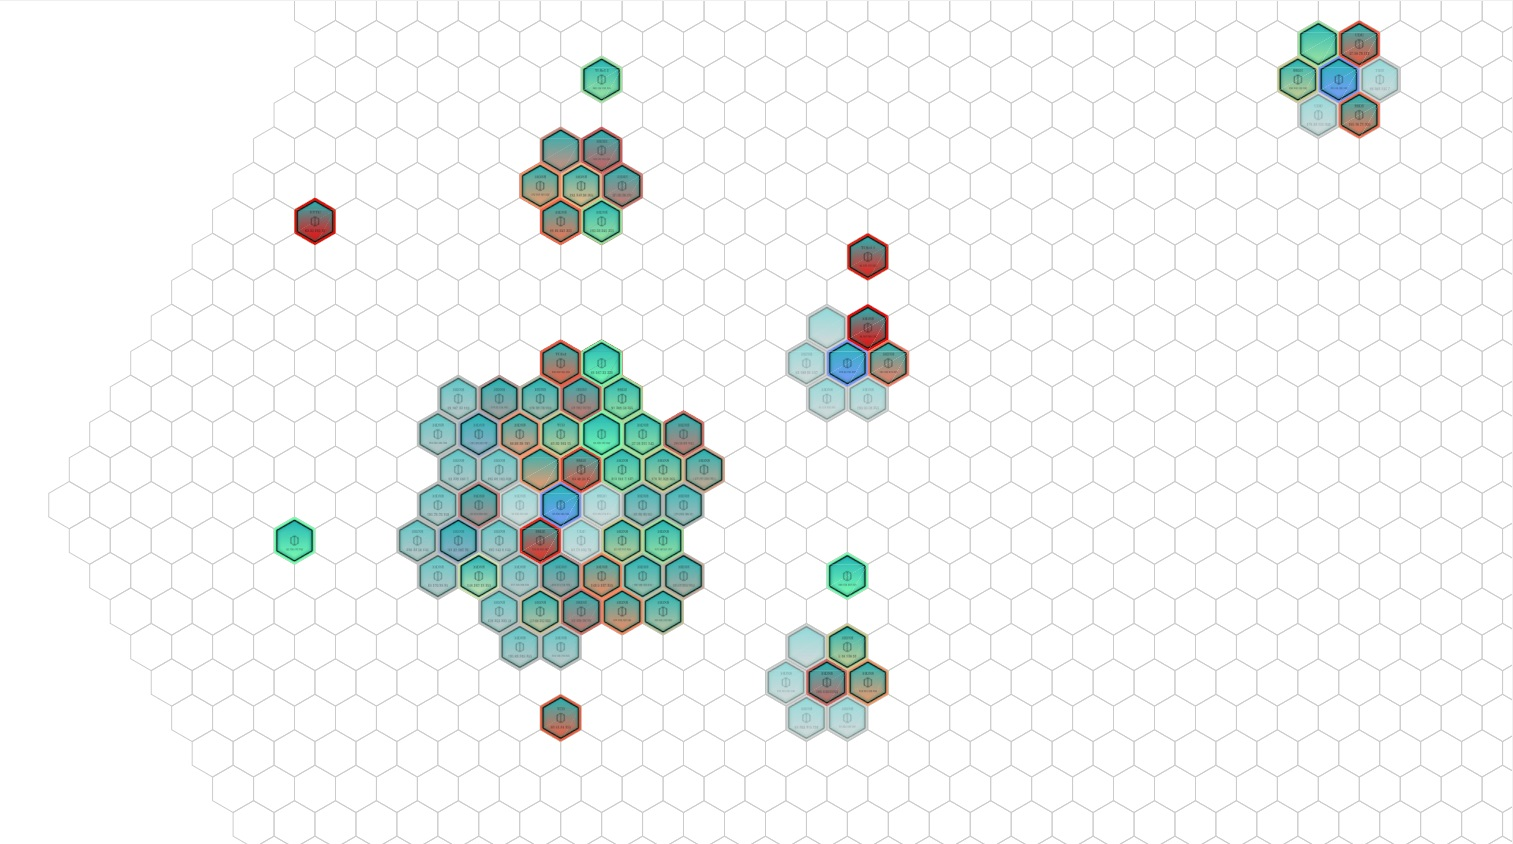
\includegraphics[width=\linewidth]{materials/groups.jpg}
   \caption[Activity Groups]{\label{fig:groups}
         Activity Groups visualization.}
\end{figure}

The colour of the communicating nodes represents how much data they send. More heavily used
destinations will thus have more orange and red nodes around them, and destinations used by a lot of
machines will have a greater number of nodes around them. Node placement is automatic. The procedure
ensures that there is enough space around a centre and that no two nodes overlap.

This visualization helps detect the machines that perform a server role in the network.
It also allows the user to quickly guess what type of service the device is providing. Each node
specifies the most commonly used protocol, thus revealing the possible role of the machine in the
network. Once the typical pattern of connections is identified, it can be filtered out to show
possible anomalies.

\section{User Workflow} \label{sec:workflow}
%From the perspective of an analyst examining a network, a typical workflow
would begin with considering all activity from a broad overview, using any
number of visualizations. Once a network attack has been identified, it should
be easy for the analyst to ``zoom in'' to the data of interest, by applying
successive filters to the source, and changing the representation to suit the
particular attack. Finally, when the exceptional behaviour has been singled
out, the analyst may explore details of the intrusion on demand.

This workflow illustrates the visual design framework suggested by Ben
Shneiderman, University of Maryland, in 1996;

\begin{center}
    \textit{Overview first, zoom and filter, then details-on-demand.}
\end{center}

To assist with the process of singling out suspicious activity, certain
visualizations allow filtering by mouse interaction. Where appropriate, the
analyst may click or drag their mouse cursor over sections of the active
visualization to create a new filter, or switch to a different representation
of the selected data. Navigation between complementing visualizations in this
fashion is highly intuitive and allows the analyst to tweak the active filters
quickly and effectively.

The following is a graphical representation of the typical workflow expected of
an analyst studying a network using NetVis.

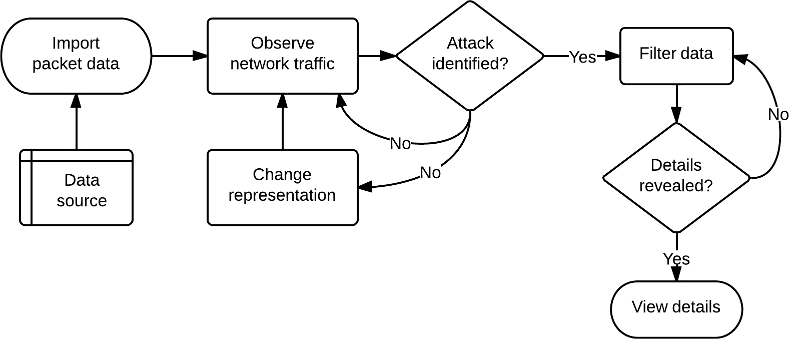
\includegraphics[width=\linewidth]{materials/workflow-diagram.png}

Our workflow can be considered an extension to the visualization workflow paradigm proposed by Ben
Shneiderman \cite{shneiderman1996designing}: \textit{`Overview first, zoom and filter, then
details-on-demand.'}. The core difference being that even an overview may have several perspectives
of the same data. By allowing several perspectives to visualize the same data simultaneously enable
analysts to explore a dataset based on their requirements and where they see patterns emerging. 

A typical workflow for an analyst would begin by considering all activity from a broad overview,
using any number of the visualizations. Once a network attack has been identified, the analyst to
``zoom in'' to the data of interest by applying successive filters to the source and changing the
representation to suit the particular attack. Finally, when the exceptional behaviour has been
singled out, the analyst may explore details of the intrusion. A diagram of the typical workflow for
an analyst using NetVis can be found in Figure \ref{fig:workflow}.

\begin{figure}[htb]
   \centering
   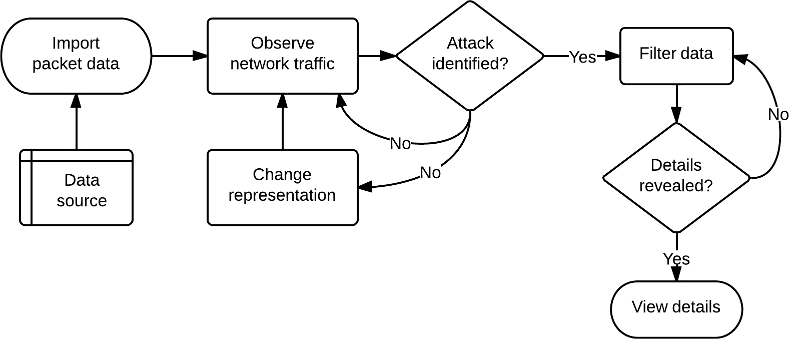
\includegraphics[width=\linewidth]{materials/workflow-diagram.png}
   \caption[Workflow]{\label{fig:workflow}
         A diagram outlining the workflow paradigm for using NetVis.}
\end{figure}

To assist with the process of singling out suspicious activity, certain visualizations allow
filtering by mouse interaction. Where appropriate, the analyst may click or drag their mouse cursor
over sections of the active visualization to create a new filter or to switch to a different
representation of the selected data. Navigation between complementing visualizations in this fashion
is highly intuitive and allows the analyst to tweak the active filters quickly and effectively.

\subsection{Example Scenarios}
To obtain a complete understanding of a network's activity, a single visualization will not
typically be sufficient. An analyst will need to see different approaches to interpret the data, and
will need to customise the visualizations and the data displayed in them. This is where the design
principles of interactivity and interconnectedness of NetVis provide powerful assistance, and ensure
that the visualizations in combination achieve both effectiveness and expressiveness
\cite{mackinlay1987automatic}. An analyst can train for detecting attacks by using packet captures.
By using a different filter combinations they are able to isolate the attack an learn more about it.
Below follows two examples of the workflow in use.

\subsubsection{Example Scenario: Portscan}
\begin{figure*}[htbp!]
	\centering
	\subfigure[A tall spike in the attribute distribution.]{
	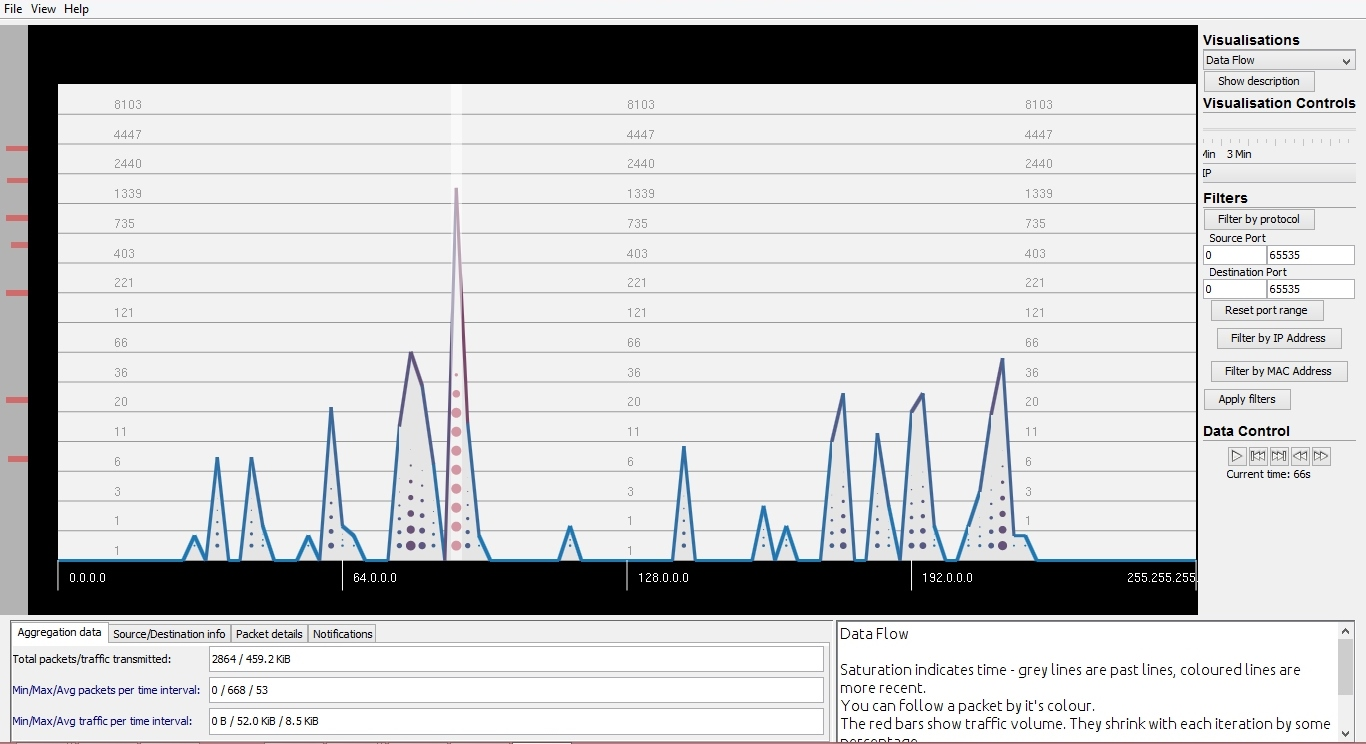
\includegraphics[width=.3\linewidth]{materials/portscan_identify}
	\label{fig:portscan0}
	}
	\subfigure[Activity suggests a portscan.]{
	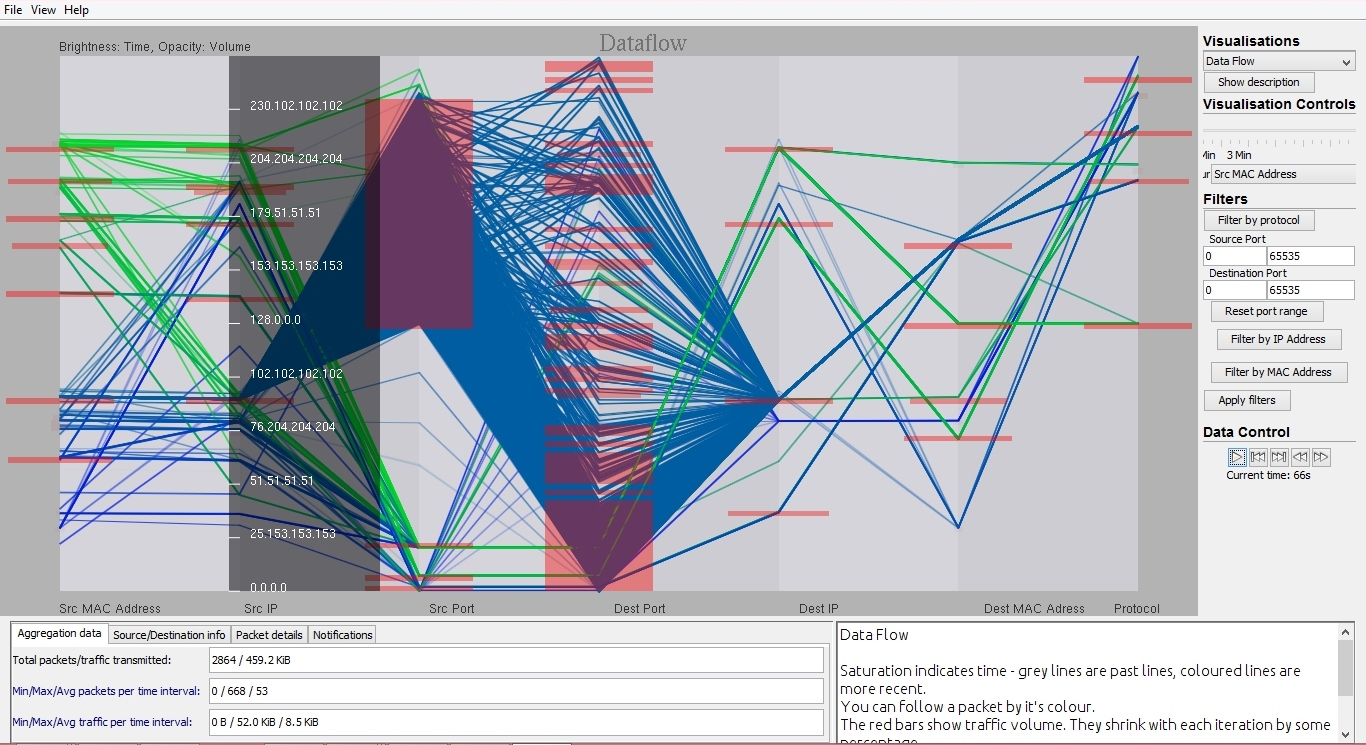
\includegraphics[width=.3\linewidth]{materials/portscan_detected}
	\label{fig:portscan1}
	}
	\subfigure[Filters show a single IP is responsible.]{
	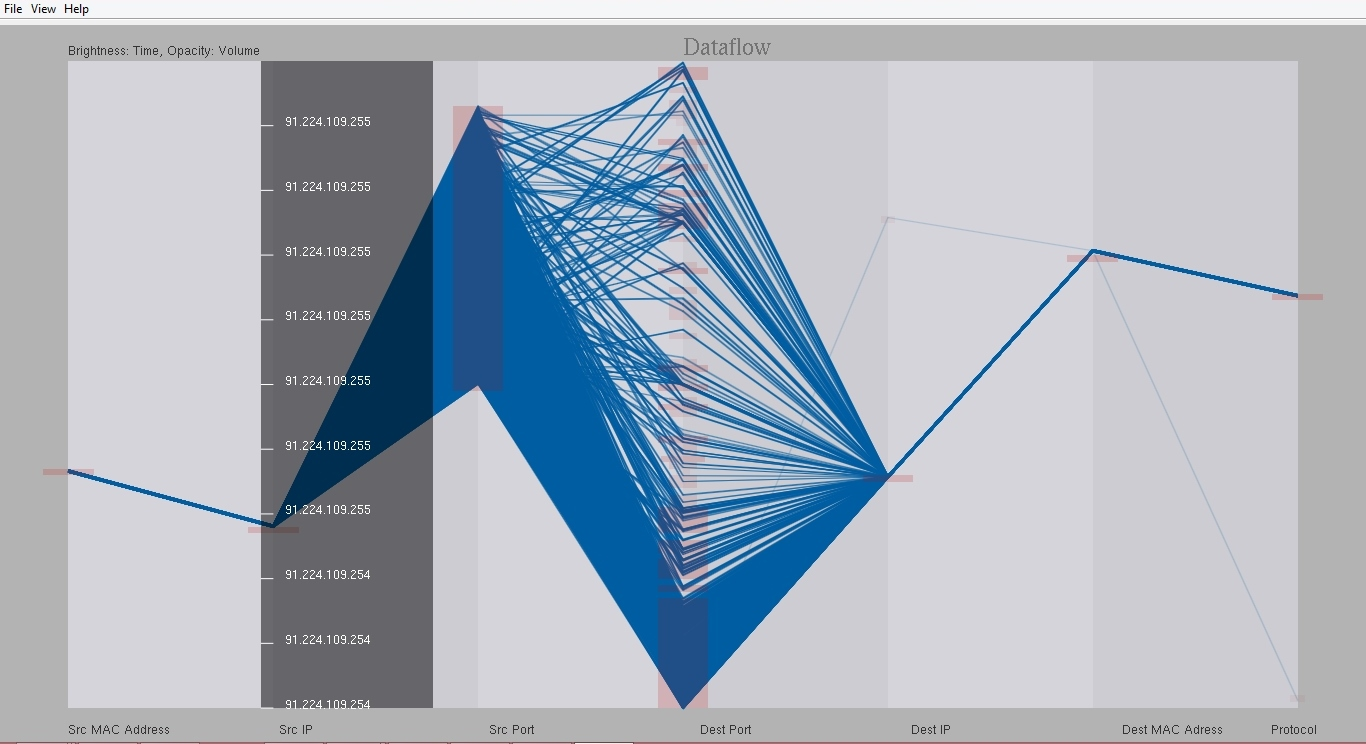
\includegraphics[width=.3\linewidth]{materials/portscan_explore}
	\label{fig:portscan2}
	}
	\caption{\label{fig:portscan} Example scenario of network portscan.}
\end{figure*}

In Figure \ref{fig:portscan0} it is possible to see a tall spike in the attribute distribution. By
visualizing the distribution of source IP's the analyst can distinguish a spike in the network
traffic for a small IP range. Clicking the spike changes the current visualization to the DataFlow
visualization, see Figure \ref{fig:portscan1}. It can then be noted that many sources may go to the
same range of ports. A filter can then be applied to isolate who is responsible for the majority
of the port activity. Figure \ref{fig:portscan2} shows the same DataFlow visualization after
applying a range filter to isolate the port scan which they can explore further in all the
visualizations. The filtering shows a single IP is responsible for the portscans.

\subsubsection{Example Scenario: SSH Brute Force Attack}
In Figure \ref{fig:ssh0} an analyst can observe some irregular activity in the traffic volume
visualization. The ongoing volume of SSH is roughly the same amount at most of the intervals. After
exploring with a couple of filters, see Figure \ref{fig:ssh1} the analyst finds out that a single IP
is responsible for all the irregularities. A quick look at the analysis panel (in the swing GUI)
provides information about the attacker and the destination. By isolating the packets from the
suspicious IP he can determine the type of attack. 

\begin{figure}[htb]
	\centering
	\subfigure[Suspicious SSH]{
	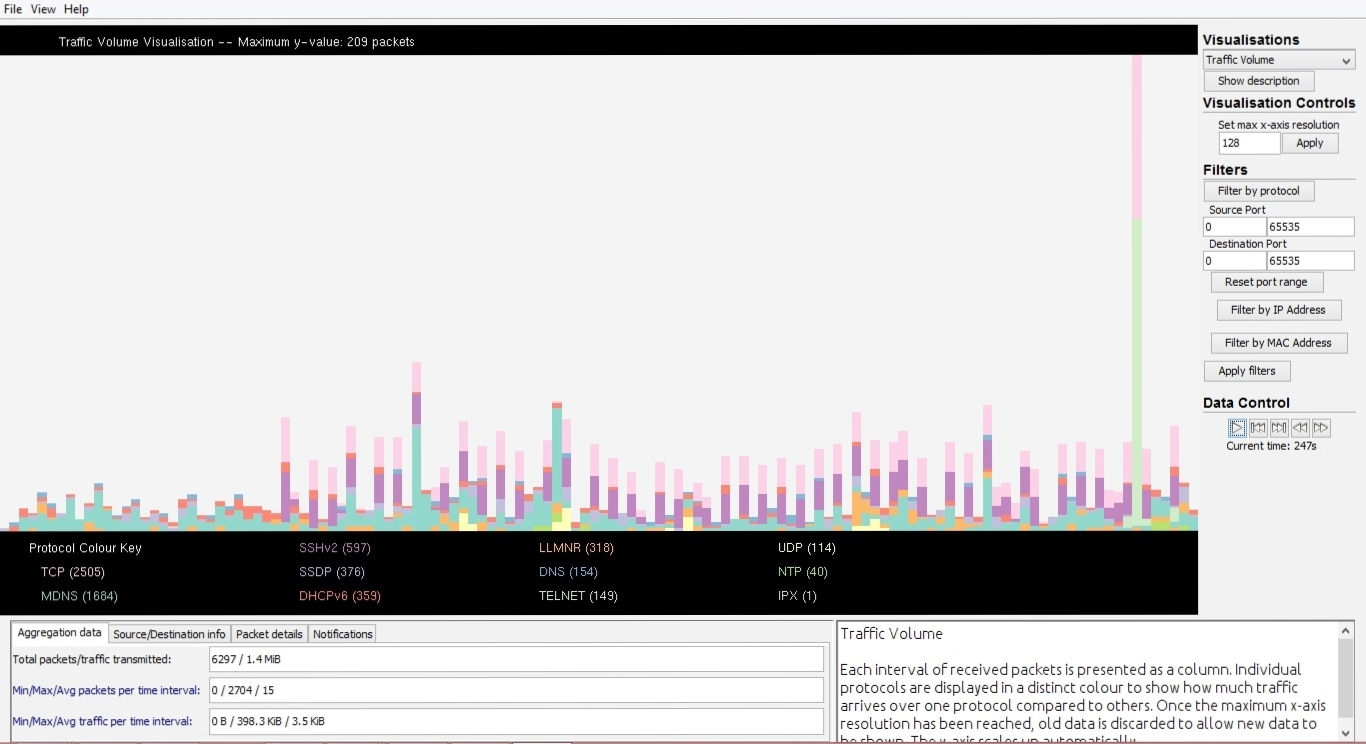
\includegraphics[width=.45\linewidth]{materials/ssh_suspicious}
	\label{fig:ssh0}
	}
	\subfigure[Exploring SSH data]{
	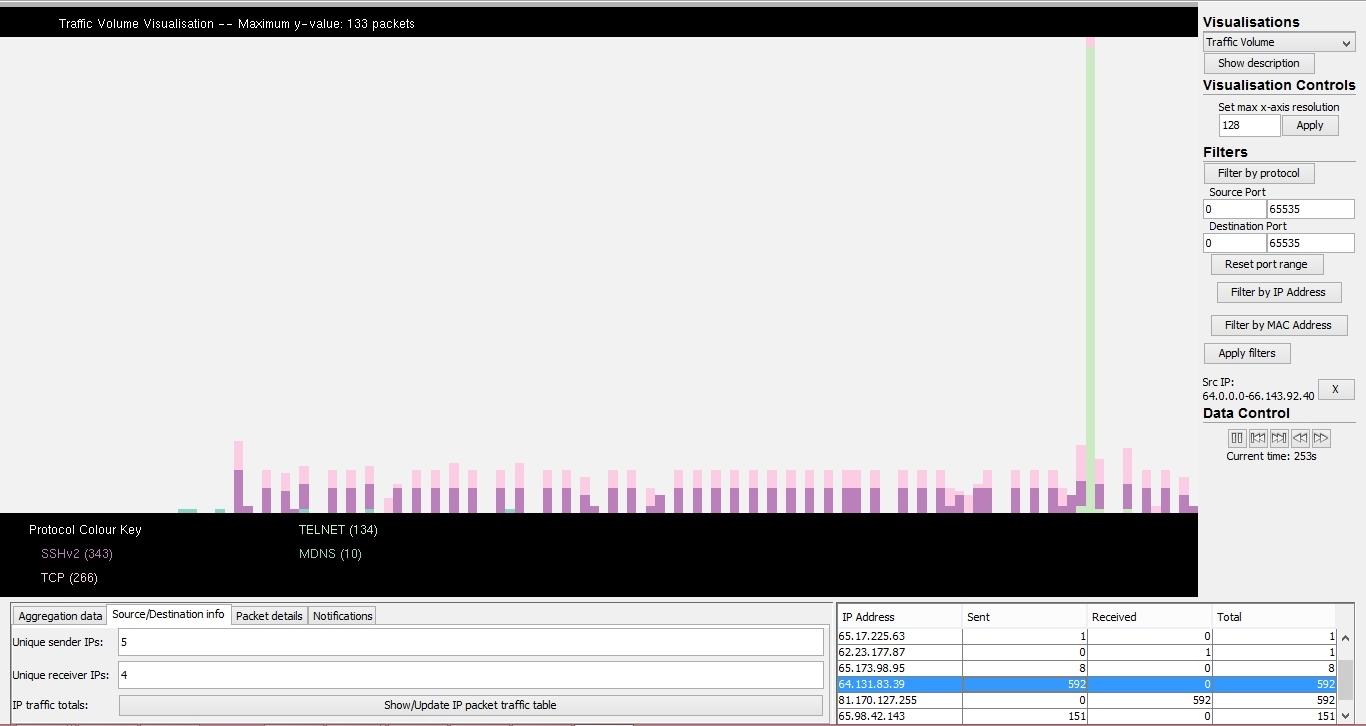
\includegraphics[width=.45\linewidth]{materials/ssh_explore}
	\label{fig:ssh1}
	}
	\caption{\label{fig:ssh} Example scenario of an SSH brute forcing.}
\end{figure}


\section{Discussion} \label{sec:discussion}
%The main determinants of traffic in a network are the network's topology, the flow of the traffic, and the type of the traffic. The graphical visualizations presented here ensure that the available data can be interpreted from all three of these perspectives. Moreover, the underlying idea of our design is that better insight into the activity in the network can be gained by combining these perspectives.

Each visualization was chosen to fill a specific purpose.  The Heat Map visualization fills the need to gain a very quick impression of overall network load and size.  The Activity Groups visualization provides the same information on a server-by-sever basis, providing more data at the expense of simplicity.  The Data Flow visualization provides the ability to see what the traffic of the network currently `looks' like, and the Spinning Cube and Attribute Distribution visualisations allow the user to detect pattern in the attributes of the packets.

Note that the visualizations combined here differ in their approach to handling the inherent multi-dimensionality of traffic data. An effective visualization framework needs to make clear how traffic changes as time progresses, and needs to show interesting developments in diverse attributes such as port use, source and destination machines, protocol use or traffic volume. Showing all this information simultaneously runs at the risk of obstructing the simplicity needed for ready understanding of a human observer. Our visualizations both use multi-dimensional systems (such as parallel coordinates) to give an overview, and use visualization with fewer dimensions but more detail. This encourages an understanding of network activity that is both broad and detailed.

To arrive at a complete understanding of the network, a single visualization will typically not be sufficient. An analyst will need to see different approaches to interpret the data, and will need to customize the visualizations and the data displayed in them. This is where the design principles of interactivity and interconnectedness of NetVis provide powerful assistance, and ensure that the visualizations in combination achieve both effectiveness and expressiveness \cite{mackinlay1987automatic}. 
Important aspects of network traffic include the network's topology, the flow of the
traffic, and the type of the traffic. The graphical visualizations presented here ensure that the
available data can be interpreted from all three of these aspects. Moreover, we believe better
insight into the activity in the network can be obtained by combining perspectives.

Each visualization fulfills a specific purpose. The Heat Map visualization provides a very quick
impression of overall network load and size. The Activity Groups visualization provides the same
information on a server-by-sever basis, providing more data at the expense of simplicity.  The Data
Flow visualization provides the ability to see what the traffic of the network currently `looks'
like, and the Spinning Cube and Attribute Distribution visualizations allow the user to detect
patterns in the attributes of the packets.

The visualizations developed here differ in their approach to handling the inherent
multi-dimensionality of traffic data. An effective visualization framework needs to make clear how
traffic changes as time progresses, and needs to show interesting developments in diverse attributes
such as port use, source and destination machines, protocol use or traffic volume. Showing all this
information simultaneously risks obstructing the simplicity needed for ready understanding. 

\subsection{Advantages}
Existing network visualization solutions are typically single-purpose programs which present given
data in one specific way (see for instance the catalogue in \cite{marty2009applied}). The analyst is
expected to choose in advance which kind of visualization will provide the most insight, and is then
limited to what the specific application is able to show. Existing applications also require
different input file formats which makes simultaneous use complicated, and sometimes impossible when
a SIEM uses proprietary middleware not commonly supported. NetVis takes a single data input stream
and simultaneously visualizes it in different presentations. Since these visualizations are built
upon a common base, they are able to complement and inform each other. This improves the user's
ability to investigate anomalies.

Network visualizations have to process and display a large amount of data. Often, this can cause a
visualization to become cluttered. An obvious solution is to provide filters which allow the analyst
to focus on phenomena of interest. The filters we provide apply application-wide and can be defined
in an intuitive manner from within the visualizations themselves in a ``click-and-zoom'' fashion.
This is a significant improvement over existing workflows.

The framework developed here can be used both for real-time monitoring and for historical analysis,
which makes it applicable to a wide variety of use cases. Furthermore, the application can be used
as a learning tool: by observing archived data captures, new users can familiarise themselves with
the general patterns of network usage and can see how suspicious patterns show up in a
visualization.

\subsection{Limitations}
Our visualizations currently only support the analysis of time series data of packet captures at the network layer. However, a multi-layer approach combined with with security event information from intrusion detection systems, routers and firewalls will likely help inform the analyst more accurately about the state of the network. The application in its current state does not analyse the content of packets. NetVis assumes domain expert users. If a user is unfamiliar with common network protocols it may be difficult for them to understand the meaning of emerging patterns. 
%Developing support for learning or showing how the protocols relate to real world consequences may help them.

\subsection{Future Work}
%More advanced data processing
Machine Learning
Save current configuration and have access to sensible filter packages

We have a number of avenues for future work. We will continue to explore the utility and
effectiveness of the framework through the growth of visualizations tools it supports and
experiments with expert users. We will extend the data types we support (to allow for the
consideration of data from other layers and security appliances) and explore the relative benefits
and limitations, seeking to identify any plateau effects (i.e. to keep vigilance levels high). We will also explore a more powerful data preprocessing system. Further, we will experiment with the application of statistical inference to the data with historical observations incorporated. Finally, it would be valuable to assess our workflow paradigm by testing it using data from outside laboratory settings and obtain comments from analysts in real environments.

\section{Conclusion} \label{sec:conc}
%We have presented a network visualization tool to analyse and monitor network traffic. Instead of presenting single perspectives (visualizations) of the data very well (but with a limited scope), our framework delivers a variety of visualizations that complement each other and work in tandem to help an analyst obtain improved awareness of ongoing network activity through user interaction. We overviewed its suite of visualizations and demonstrated its usefulness with example scenarios. In the future we intend to add more visualizations and further improve the tool's usability.

We have presented a network visualization tool to analyse and monitor network traffic. Instead of
presenting single perspectives (visualizations) of the data very well (but with a limited scope),
our framework delivers a variety of visualizations that complement each other and work in tandem to
help an analyst obtain improved awareness of ongoing network activity through user interaction. We
overviewed its suite of visualizations and demonstrated its usefulness with example scenarios. In
the future we intend to add more visualizations and further improve the tool's usability.

%-------------------------------------------------------------------------
\bibliographystyle{eg-alpha}
\bibliography{netvisbib}

\end{document}
